\documentclass[assd_tp2_main.tex]{subfiles}

\begin{document}

\section{Síntesis mediante modulación en frecuencia}
\subsection*{}
La modulación en frecuencia esta dada por:
\begin{eqnarray*}
\textstyle x(t)=A(t)cos(2\pi f_c t+I(t)cos(2\pi f_mt+\phi_m)+\phi_c)
\end{eqnarray*}
Parámetros de la modulación en frecuencia:
\begin{eqnarray*}
\displaystyle c, m, d  \\* I=\frac{d}{m}  
\end{eqnarray*}
Donde: \\*
c = frecuencia de la señal portadora\\*
m = frecuencia de la señal modulante\\*
d = desviación de la frecuencia\\*
\\
Por simple inspección se puede ver que si I = 0 la desviación de la frecuencia (d) debe ser 0 y por ende no hay  modulación en frecuencia. Un caso más interesante es cuando I es mayor que 0, se puede observar que aparecen nuevas componentes espectrales lo que provoca que la energía de la señal sea redistribuida.  
\begin{figure}[h!]
\centering
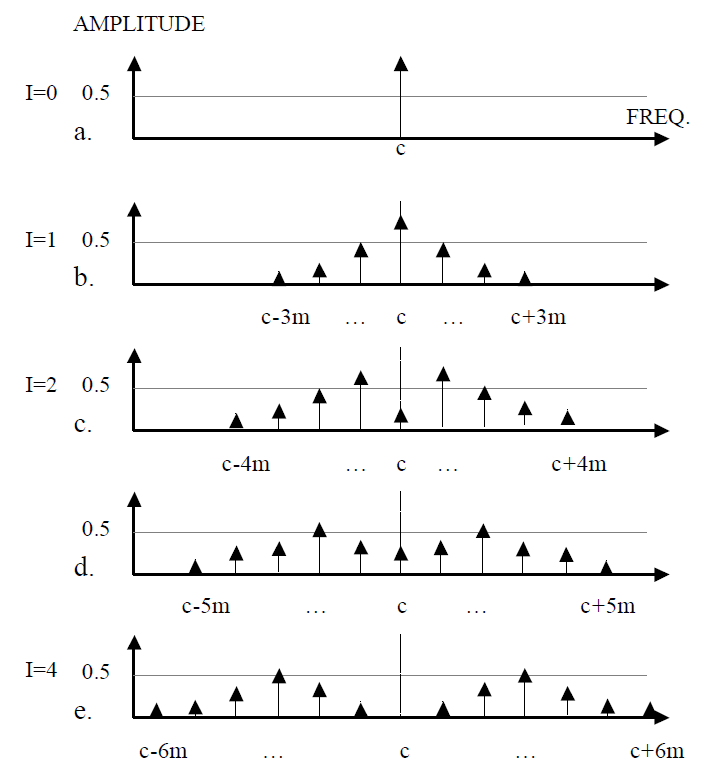
\includegraphics[width=0.4\linewidth]{nuevasfreqs.png}
\caption{Nuevo contenido espectral con I $\neq$ 0}
\label{fig:nuevasfreqs}
\end{figure}
Las amplitudes de la portadora y las componentes laterales están dadas por las funciones de Bessel de primera especie y orden n-ésimo,
donde el argumento de la función es el índice de modulacion I ($J_{n}$(I)). \\*
En general, $J_{n}(1)$ representa un coeficiente de escalamiento de amplitud: \\*

$J_{0}(1)\longleftarrow$  para la portadora \\*

$J_{1}(1)\longleftarrow$  para las primeras bandas laterales \\*

$J_{2}(1)\longleftarrow$  para las segundas bandas laterales \\*
\\*
Y así sucesivamente.
\todo[inline]{No entendi a lo que se refiere con: .\newline The higher the order of the side frequency the larger the index must be for that side frequency to have significant amplitude \newline y que onda con el BW como paso eso}

El bandwidth total es aproximadamente igual a
\begin{eqnarray*}
\displaystyle BW \approx 2(d+m)
\end{eqnarray*}

Expresamos a x(t) con funciones de Bessel
\begin{eqnarray*}
\textstyle x(t)=A(t)\cdot \{ \; J_{0}(I)sen(2\pi f_c t) \\*
				+J_1(I)[sen(2\pi(f_c+f_m)t) - sin(2\pi(f_c-f_m)t)] \\*
				+J_2(I)[sen(2\pi(f_c+2f_m)t) + sin(2\pi(f_c-2f_m)t)] \\*
				... \\*
				+J_n(I)[sen(2\pi(f_c+n f_m)t) - sin(2\pi(f_c-n f_m)t)] \; \}
\end{eqnarray*}
Se puede ver que las bandas laterales bajas de orden impar poseen un signo negativo que provoca que para para un I>2.5
las funciones de bessel produzcan coeficientes de escalamiento negativos para algunos componentes.
En general se suelen ignorara los signos negativos en el espectro ya que solo indican una inversion de la fase de la frecuencia correspondiente.
\todo[inline]{Poner foto de espectro con la fase, flecha para abajo y quiza poner alguno para mostrar lo de I>2.5}


\subsection*{Frecuencias laterales reflejadas}
La riqueza de esta técnica yace en que el espectro ubicado en la parte negativa del dominio interfiere con la parte positiva dando lugar a una mezcla de componentes en ambas partes del espectro. La relación entre frecuencias es la que da origen en este caso al espectro harmónico y inharmonico.
\subsection*{Espectro harmónico e inharmónico}
La relación entre frecuencias esta dada por \\*

\begin{eqnarray*}
\displaystyle \frac{f_c}{f_m}=\frac{N_1}{N_2} 
\end{eqnarray*}
 
\begin{eqnarray*}
\displaystyle f_0=gcd(f_c,f_m)
\end{eqnarray*}
 
La posición de las frecuencias laterales en serie harmónica puede ser determinada por las siguientes relaciones

\begin{eqnarray*}
\displaystyle k = N_1 + nN_2 \: para\; n\;\epsilon \mathbb{N}
\end{eqnarray*}
Donde k es el  número de harmónico y n es el orden de la frecuencia lateral.
Excepto para n=0, k toma dos valores por cada orden.

A continuación dejamos unas generalizaciones útiles:
\begin{itemize}
\item La portadora es siempre el $N_1$-ésimo harmónico  en la serie
\item Si $N_2$ = 1 el espectro contiene todos los harmonicos	y el fundamental es la frecuencia de la modulante
\item Si $N_2$ es un numero par el espectro tiene solo harmónicos impares
\item Si $N_2$ = 3 cada tercer harmónico no se encuentra más en la serie
\end{itemize}
 

El número de harmónicos que tienen amplitud significante  dependen del índice de modulación.

Para relaciones entre frecuencias bajas e indices chicos donde $N_1\neq1$ la fundamental puede no estar presente en el espectro.
\todo{aca tira una foto de relacion 4:1}
La fundamental solo se vuelve significante cuando I>2.\\*
Resumen:\\*
El espectro inharmónico se origina cuando el cociente c/m da como resultado un número irracional. \\*
El índice de modulación d/m determina el número de componentes que van a tener amplitud significante.

\subsection{Espectro dinámico}
La complejidad del espectro esta relacionada con el índice de modulación de forma tal que si el indice crece el bandwidth también crece. Entonces si pensamos en un índice de modulación que varía con el tiempo la evolución del bandwidth del espectro puede estar generalmente descrita por la forma de la función.
No obstante, la evolución de cada componente es determinado por la forma de la funcion de Bessel correspondiente.
Entonces, si el indice de modulación aumenta con el tiempo el bandwidth también lo hace, pero un componente del espectro va a crecer o decrecer en amplitud dependiendo de la pendiente de la función de bessel en ese rango de indices.

\todo{foto de modulacion en tiempo}



Para los intrumentos de viento:
\begin{eqnarray*}
\displaystyle \phi_m=\phi_c=-\frac{\pi}{2}
\end{eqnarray*}
Resultando
\begin{eqnarray*}
\textstyle x(t)=\textcolor{blue}{A(t)}\cdot sen(2\pi f_c t+\textcolor{magenta}{I(t)}\cdot sen(2\pi f_mt))
\end{eqnarray*}



 
\begin{eqnarray*}
\displaystyle f_0=gcd(f_c,f_m)
\end{eqnarray*}

\subsection{Síntesis de clarinete}
Para un clarinete se utiliza un esquema similar al ADSR con Attack Sustain y Release. En lugar de tratarse de una interpolación lineal entre puntos, se trata de una interpolación exponencial.

\subsection{Síntesis de campana}
Para una campana se suele utilizar

\end{document}
